\documentclass{article}
\usepackage{graphicx}

\begin{document}

\title{Homework Submission Servlet Working Specification}
\author{Mike Burns}
\date{\today}

\maketitle

\section{User Interface}\label{sec:ui}

\begin{figure}[ht]
\centering
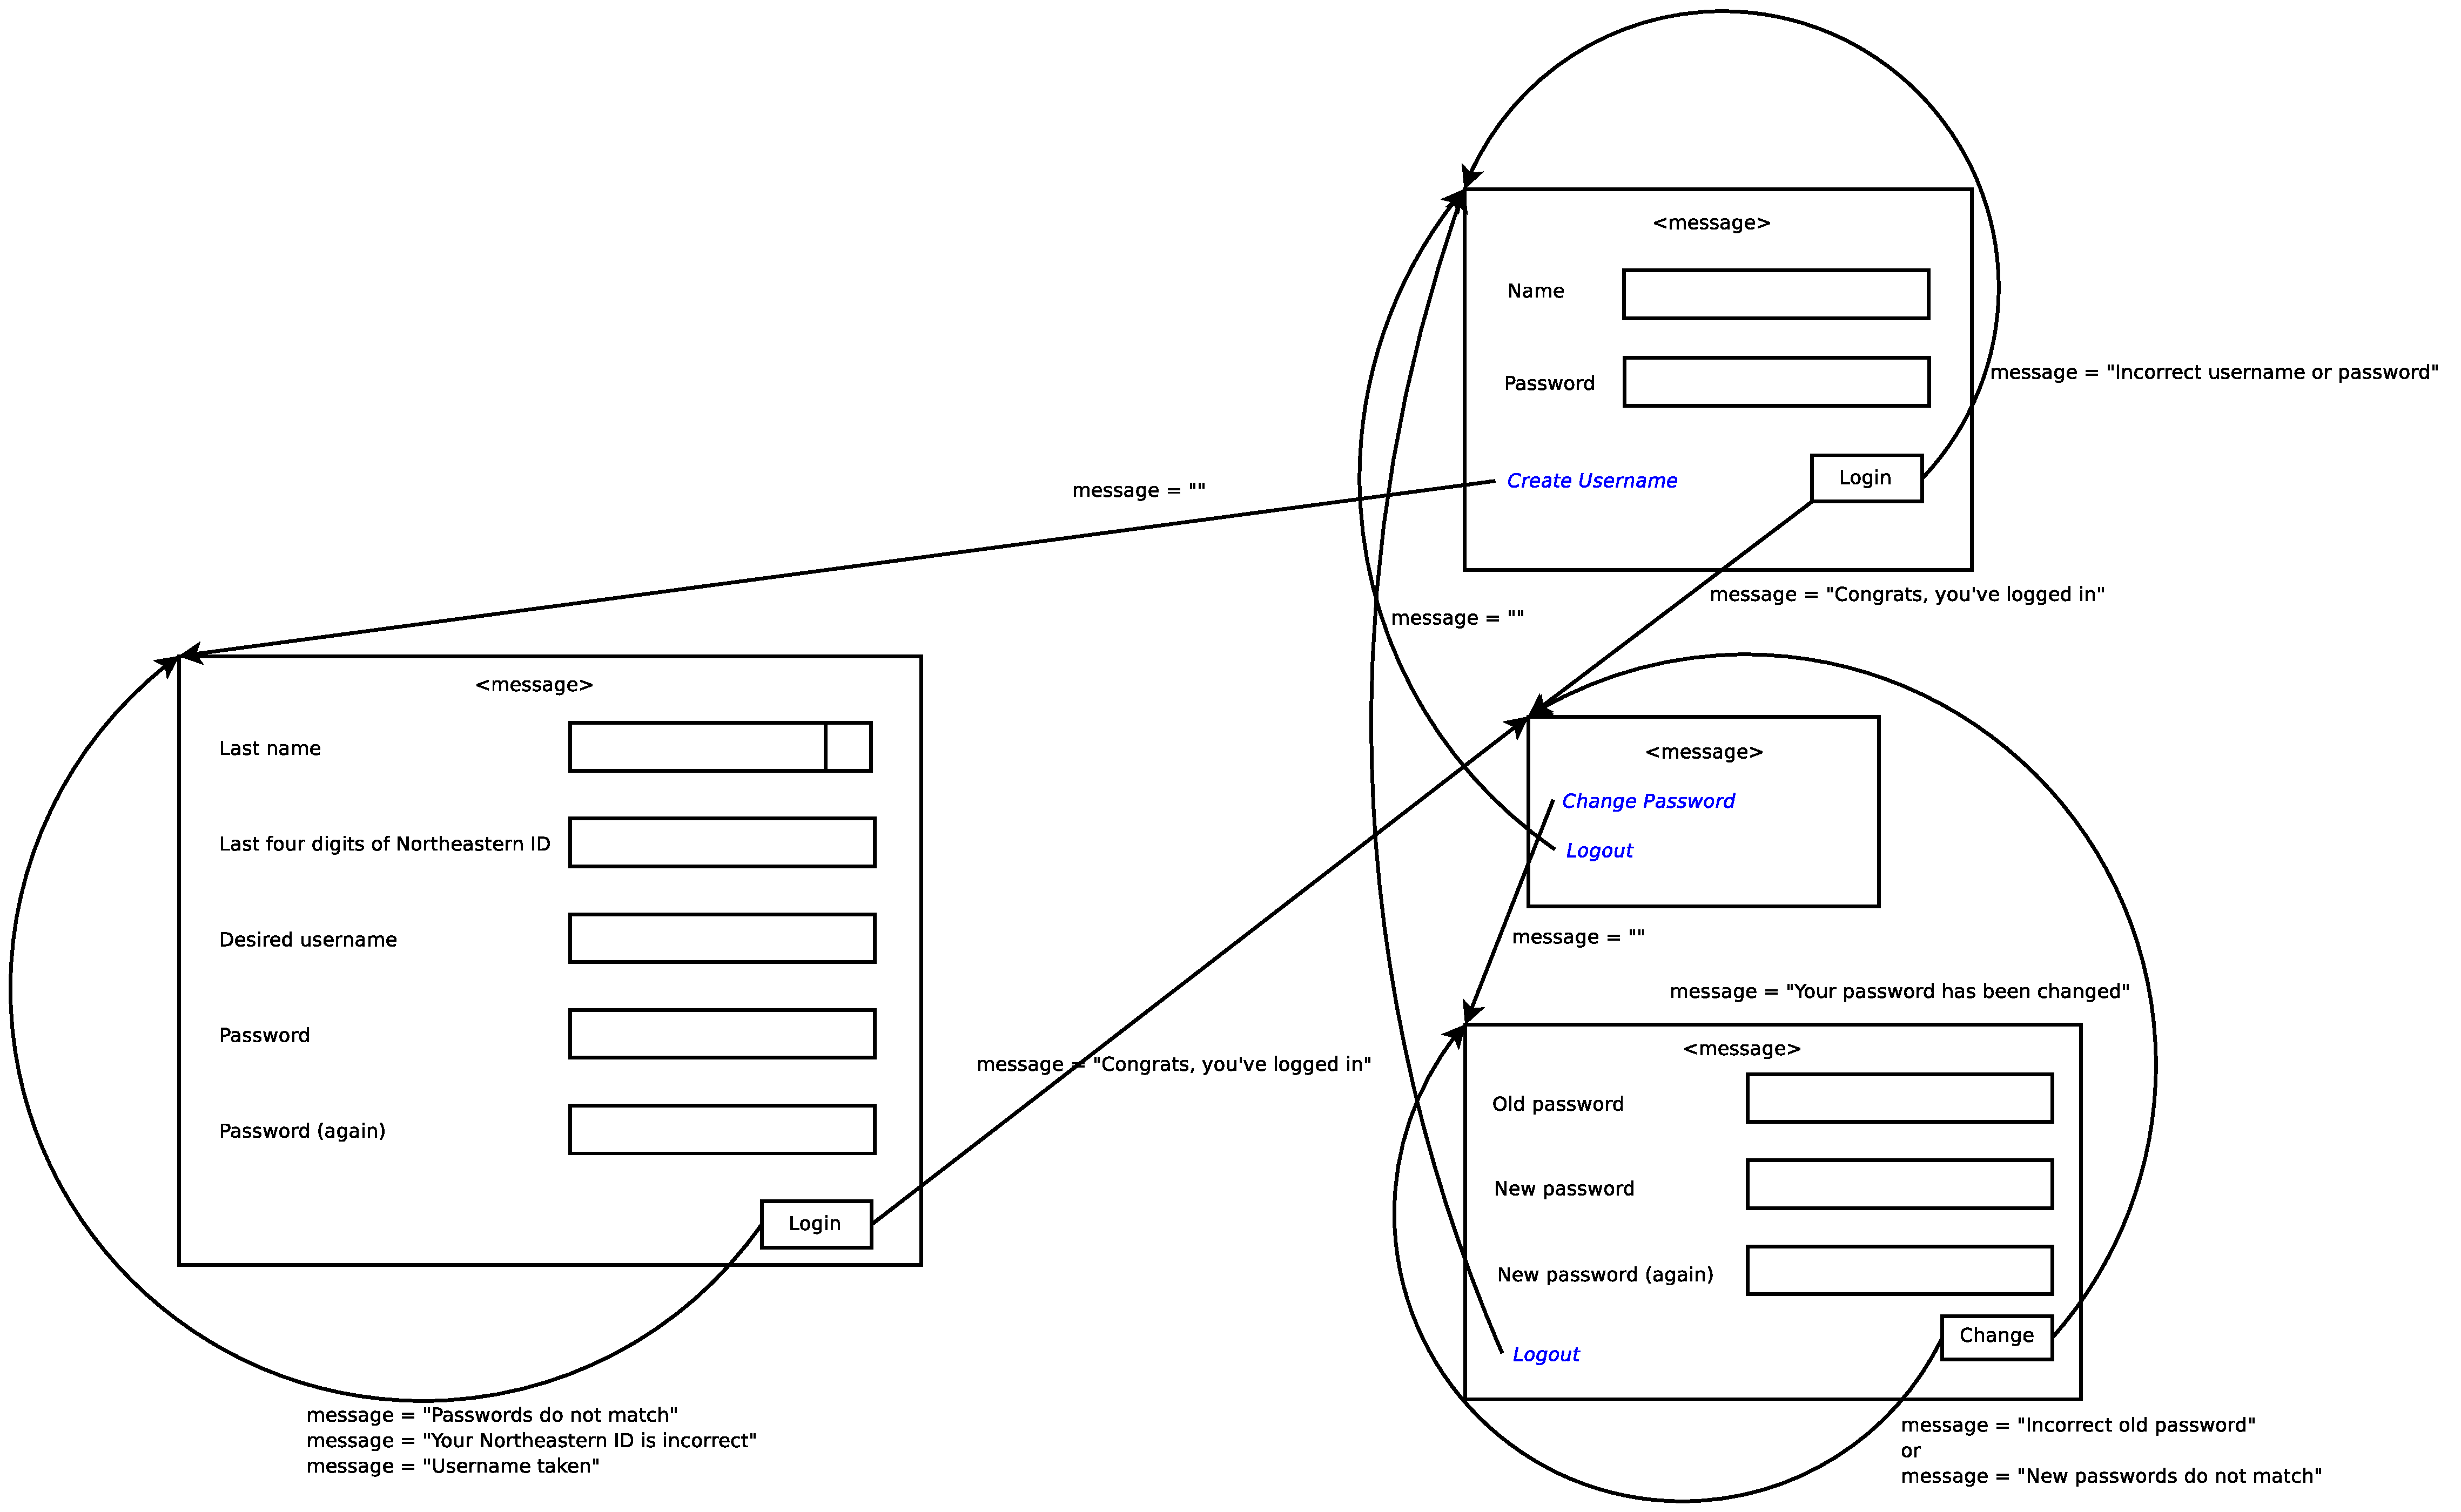
\includegraphics[scale=.35]{servlet.eps}
\caption{The servlet user interface, with interactions}
\label{fig:ui}
\end{figure}

\section{Use Cases}\label{sec:usecases}

\begin{itemize}
\item{A user enters an invalid username and/or password pair.}
\item{A user logs in, then logs out.}
\item{A user logs in, then closes the Web browser.}
\item{A user logs in, logs out, uses the back button once, then logs out again.}
\item{A user logs in, sucessfully changes his or her password, then logs out.}
\item{A user logs in, attempts to change his or her password, enters an invalid
old password, then logs out.}
\item{A user logs in, attempts to change his or her password, enters an invalid
old password, sucessfully enters the correct data and changes his or her password,
then logs out.}
\item{A user logs in, attempts to change his or her password, enters mismatched
new passwords, then logs out.}
\item{A user logs in, attempts to change his or her password, enters mismatched
new passwords, sucessfully enters the correct data and changes his or her password,
then logs out.}
\item{The Web server is restarted by the TA or instructor.}
\item{The password file is edited, with the server stopped, by the TA or
instructor.}
\end{itemize}

\section{Architecture}\label{sec:arch}

\begin{figure}[ht]
\centering
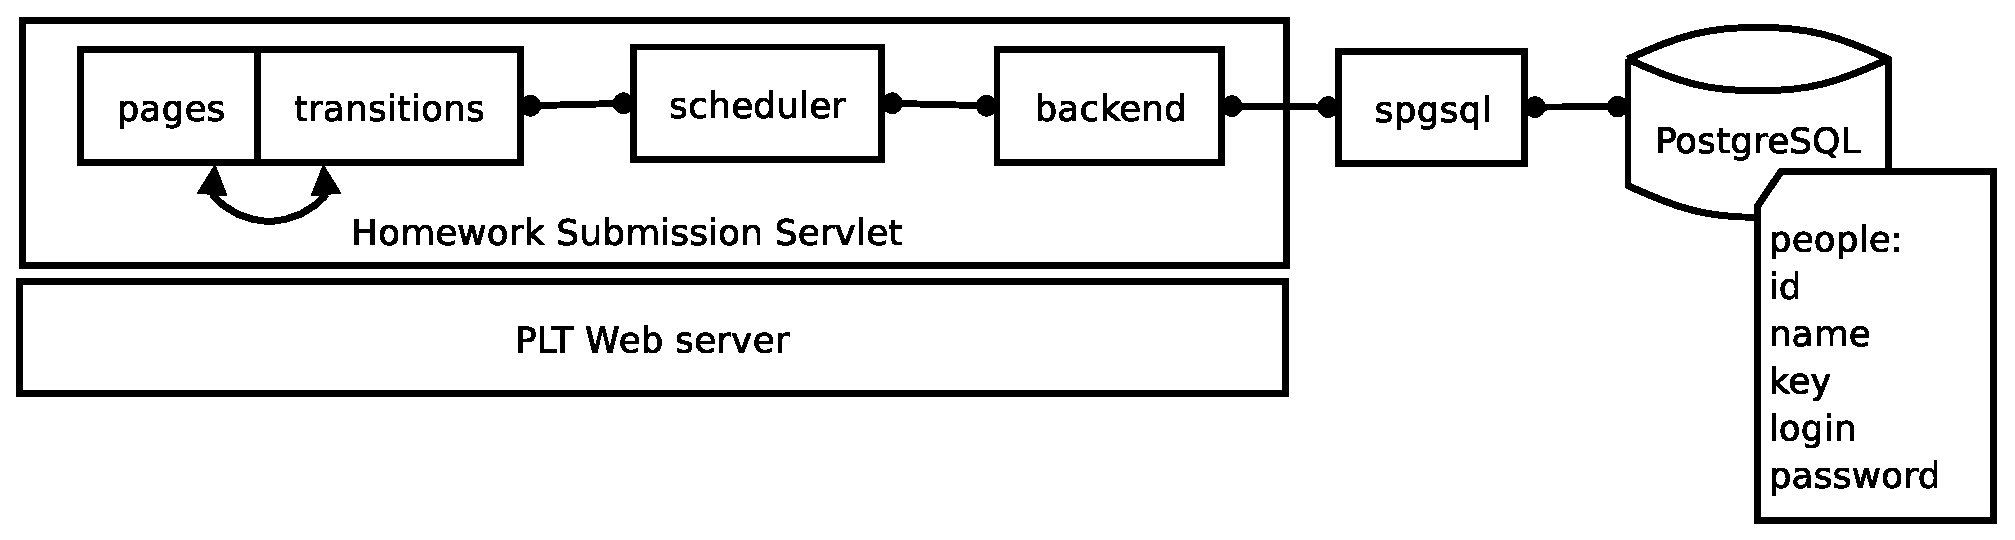
\includegraphics[scale=.35]{architecture.eps}
\caption{The high-level view of the homework submission servlet}
\label{fig:architecture}
\end{figure}

\begin{figure}[ht]
\centering
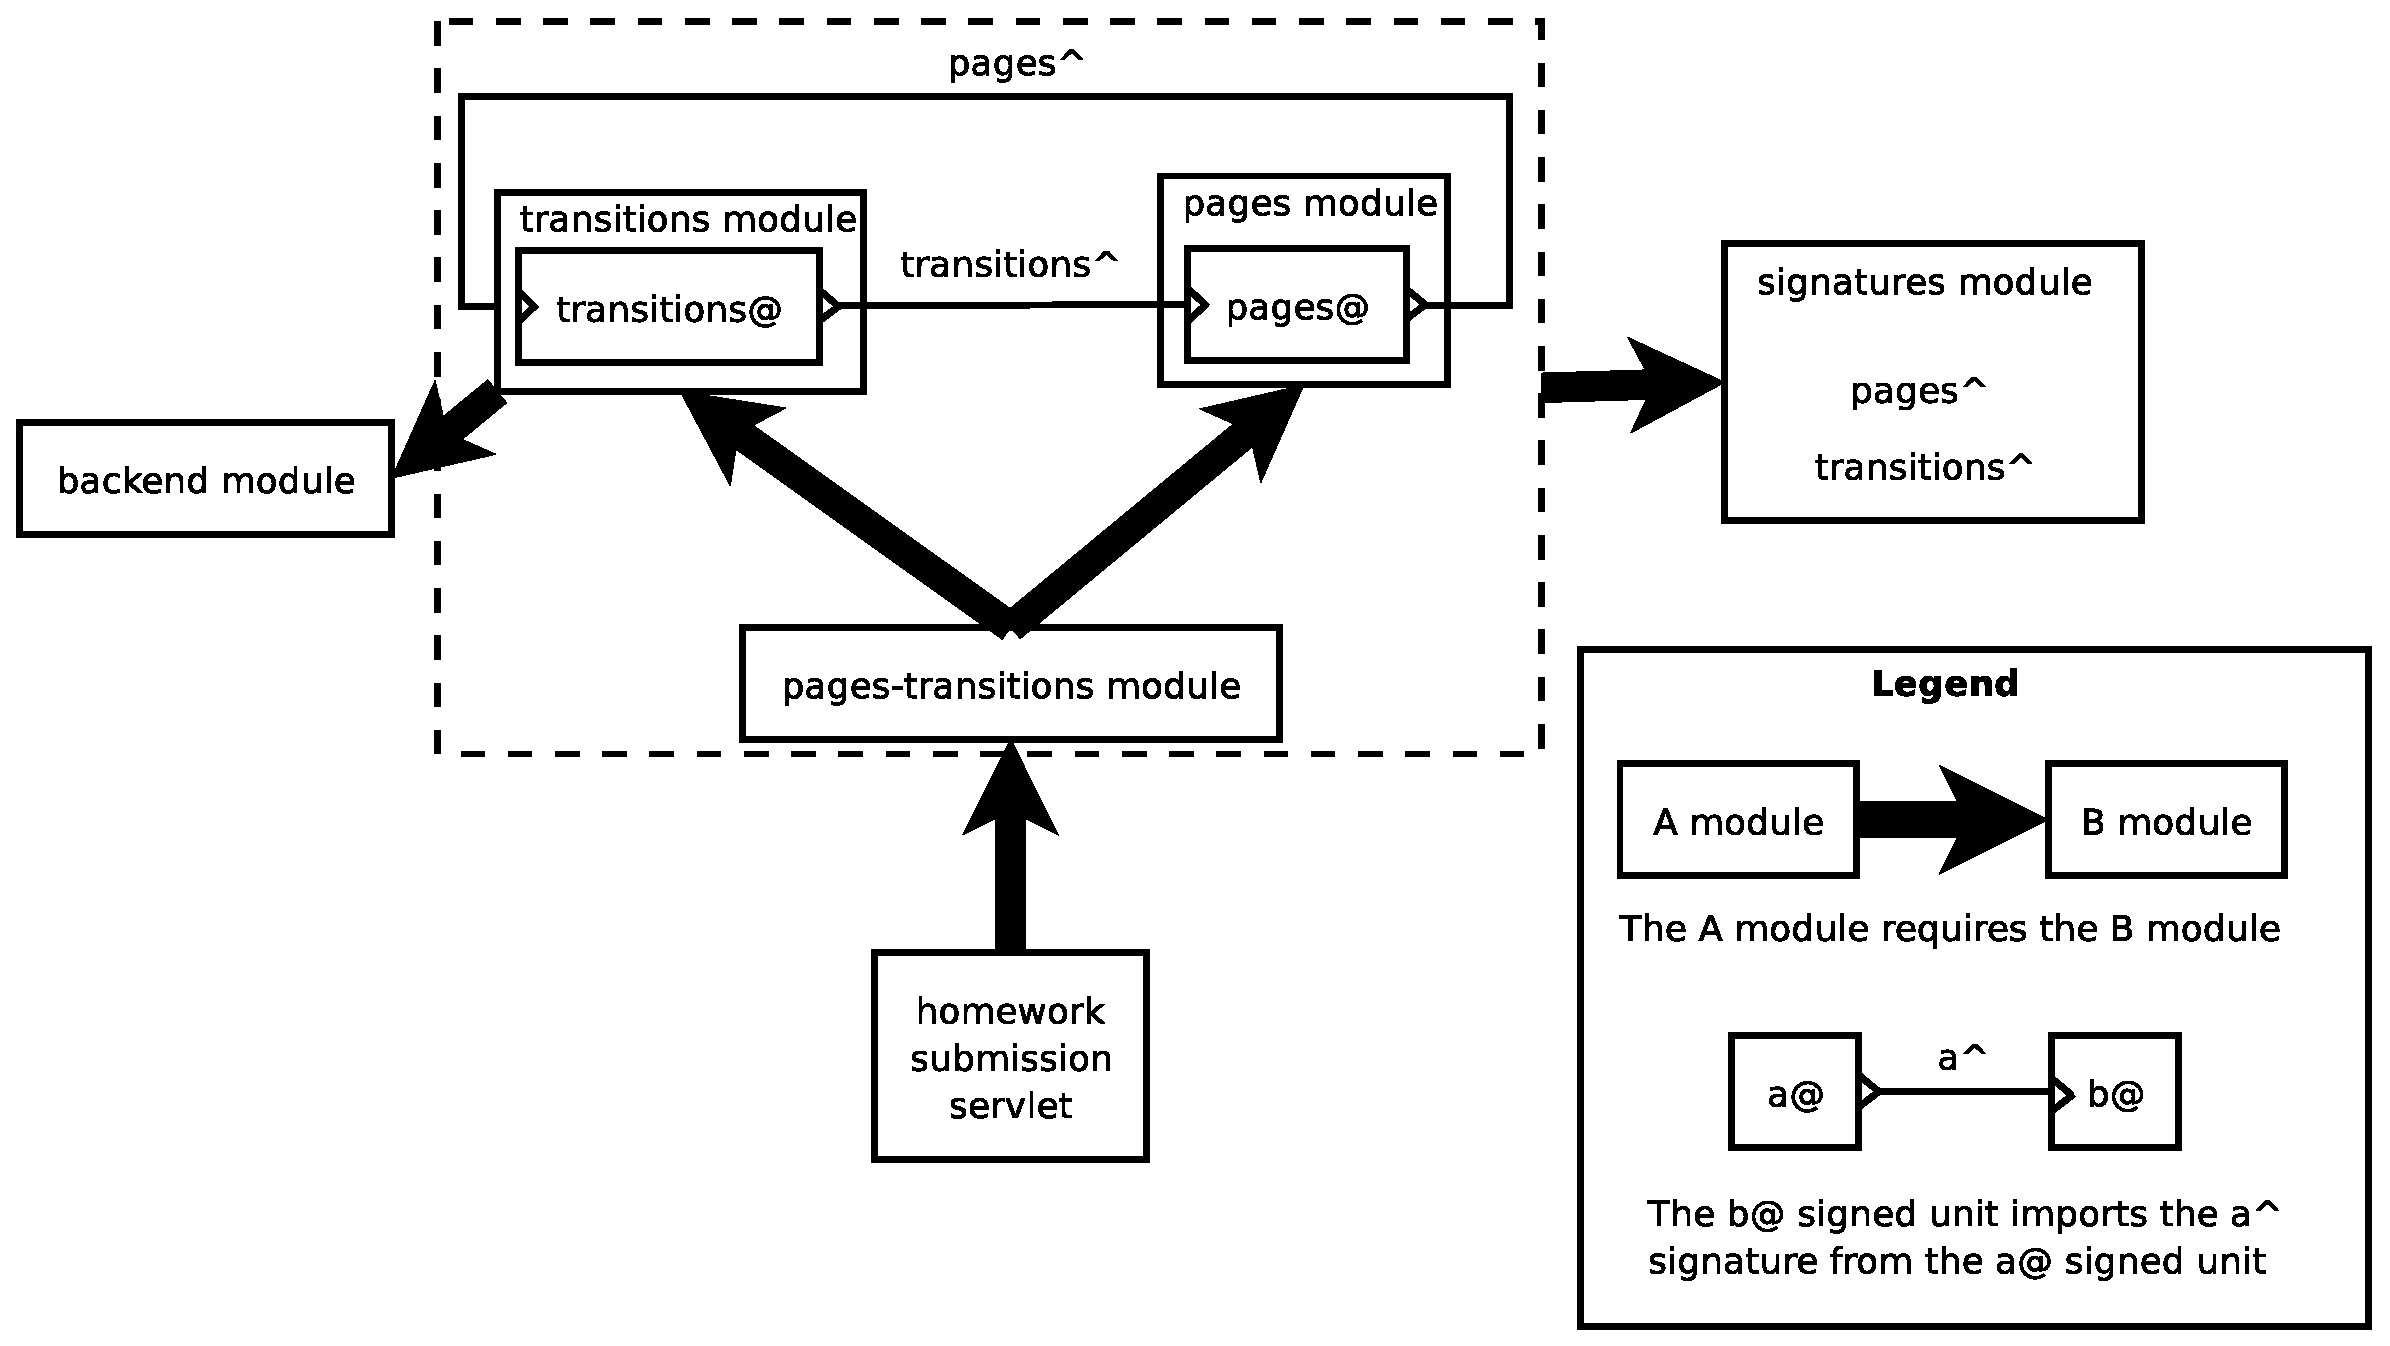
\includegraphics[scale=.35]{design.eps}
\caption{The module and unit layout of the homework submission servlet}
\label{fig:layout}
\end{figure}

The homework submission servlet is driven by the PLT Web server. It is a simple
program that calls the initial transition to send the initial login page to
the client (Web browser).

The module \verb|pages-transitions| handles the contents of the actual Web
pages and the transitions between them. It invokes and provides all from the
signed units \verb|pages@| and \verb|transitions@|.

The functions defined in the \verb|pages@| signed unit are
\verb|xexpr/callback|; that is, they are Web pages with embedded procedures.
These embedded procedures (``transitions'') have the contract\\
\verb|(request?  . -> . (union xexpr? xexpr/callback?))|.

The functions provided from the \verb|pages^| signature are

\begin{verbatim}
page-login : (() (xexpr?) . opt-> . xexpr/callback?)
Prompt the user for his or her username and password.
\end{verbatim}

\begin{verbatim}
page-logged-in :  ((session?) (xexpr?) . opt-> . xexpr/callback?)
Confirm the user has logged in.
\end{verbatim}

\begin{verbatim}
page-change-password : ((session?) (xexpr?) . opt-> . xexpr/callback?)
Prompt the user for a new password.
\end{verbatim}

Pages follow the template:

\begin{verbatim}
(define (page-foo ...)
 `(html (head (title ...))
    (body (h1 ...)
      ...
      (a ((href ,(transition-bar ...))) "Bar")
      ...)))
\end{verbatim}

Transitions are defined in the \verb|transitions@| signed unit. These are the
procedures embedded in the pages, defined in the \verb|pages@| signed unit. The
procedures provided from the \verb|transitions^| signature are

\begin{verbatim}
transition-login : (request? . -> . xexpr/callback?)
Direct transition to the login page.
\end{verbatim}

\begin{verbatim}
transition-log-in : (request? . -> . xexpr/callback??)
Action transition to the logged-in page.
Action: Check that the username and password pair are correct.
If the username and password match, send page-logged-in;
otherwise send page-login with a message.
\end{verbatim}

\begin{verbatim}
transition-log-out : (request? . -> . xexpr/callback?)
Direct transition to the login page. This clears the previously-
stored continuations first.
\end{verbatim}

\begin{verbatim}
transition-change-password : (session? (request? . -> . xexpr/callback?))
Direct transition to the change-password page.
\end{verbatim}

\begin{verbatim}
transition-update-password : (session? . -> .
                               (request? . -> . xexpr/callback?))
Action transition to the change-password page.
Action: Change the password.
Send the change-password page with a message explaining whether
it worked and, if it failed, why.
\end{verbatim}

Servlets are run in multiple threads to support multiple users; however, each
thread must access the single passwords data base as a shared resource,
creating a requirement to synchronize between threads.

Semaphores interact poorly with the timeouts maintained by the Web server, as
demonstrated in the following scenerio: the servlet grabs a semaphore, then the
Web server's timer goes off. The Web server's timer kills the servlet, which
never has a chance to post to the semaphore. This locks the servlet until it is
manually refreshed.

Instead of semaphores, we use a scheduler based on channels. All actions are
passed through the scheduler, which writes to a global scheduler channel.
These actions are read from the global scheduler channel sequentially and
executed, with their results placed on an asynchronous result channel.

The scheduler thread is started before the servlet enters the start state. It
reads, from a channel, a pair containing the thunk to execute and the
asynchronous result channel; it then executes the thunk and puts it on the
asynchronous result channel; then, it loops. The Web server's timer does not
kill this thread because it is started before the servlet enters the starting
state. 

The \verb|schedule| form creates an asynchronous result channel and puts it and
the thunk on the scheduling channel. It then reads the result from the result
channel and produces it.

Transition procedures have the form:

\begin{verbatim}
(define (transition-foo ...)
  (lambda (req)
    (let* ((a (schedule (lambda () (backend-a)))) ...)
      (send/suspend/callback (page-foo a)))))
\end{verbatim}

The backend module provides procedures only used by the procedures defined in
the \verb|transitions@| signed unit. These procedures affect the database by
selecting data from, inserting data into, or updating data in the data base.

The data base is a simple file containing a data structure with the contract
\verb|(listof (list/c string? string?))|. The first string is the username, the
second string the MD5-encrypted password. The username must be unique.


\section{Testing}\label{sec:tests}

The simulated server framework uses existing Web server modules to create its
own server, then drives the servlet through this server.

%%% 1. Clean up interface for framework
%%% 2. Document
%%% 3. Replace this will a reference to the documentation from (2).

The following tests must pass, using the simulated server framework:

\begin{itemize}
\item{A user enters an invalid username and/or password.}
\item{A user logs in, then logs out.}
\item{A user logs in, then closes the Web browser.}
\item{A user logs in, logs out, goes back to the logged-in page, and logs out
again.}
\item{A user logs in, sucessfully changes his or her password, then logs out.}
\item{A user logs in, attempts to change his or her password, enters an invalid
old password, then enters mismatched new passwords, then sucessfully changes his or
her password, then logs out.}
%%% Intentionally not tested
%\item{The password file is modified to add a user.}
%\item{The password file is modified to remove a user.}
%\item{The password file is corrupt.}
\end{itemize}

%%% Note yet done. Not sure how best to do this, either.
In addition, the script to start and stop the Web server must work for all TAs
and instructors.

\subsection{Stress Testing}\label{subsec:stresstests}

The stress-test suite drives the servlet using HTTP. This is accomplished with
\verb|get-pure-port| and \verb|call/input-url|, both from the \verb|url.ss|
module in the \verb|net| collection.

Stress tests will demonstrate potential problems this servlet will have in a
real-life situation, where many hundreds of users will be using this servlet
at once.

\subsubsection{Memory Stress}\label{subsubsec:mem-stress}

These tests will be run in an unbounded loop, in an attempt to show any memory
leaks and high memory usage in places where the servlet can not clean up after
itself.

\begin{itemize}
\item{A user logs in, then closes the Web browser.}
\end{itemize}

\subsubsection{Concurrency Tests}\label{subsubsec:parrallel-stress}

These tests will be run in parrallel with themselves, in an unbounded loop.

\begin{itemize}
\item{A user logs in, changes his or her password, then logs out.}
\item{Test the scheduler against timeouts.}
\end{itemize}

%An hourly automated test will be run against the live servlet; if this test
%fails, an email notification will be sent and the Web server restarted.

\section{Documentation}\label{sec:docs}

The documentation provided with this servlet are this outline and three
documents each describing typical use cases for instructors, teaching
assistants, and students, respecitively.

\end{document}
